% !TEX root = ../om_ts_01.tex

\begin{frame} % название фрагмента

\videotitle{Простейшие модели}

\end{frame}



\begin{frame}{Простейшие модели: план}
  \begin{itemize}[<+->]
    \item Белый шум. 
    \item Независимые наблюдения.
    \item Случайное блуждание.
  \end{itemize}

\end{frame}

\begin{frame}{Белый шум}

\begin{block}{Белый шум}
Временной ряд $u_t$ — белый шум, если:
\begin{itemize}
  \item $\E(u_t) = 0$;
  \item $\Var(u_t) = \sigma^2$;
  \item $\Cov(u_s, u_t) = 0$ при $s\neq t$.
\end{itemize}
\end{block}

\pause
\begin{itemize}[<+->]
  \item Составная часть всех моделей. Чаще всего белый шум — это, что отказались моделировать. 
  \item Часто дополнительно предполагают \alert{независимость} и \alert{нормальность}. 
  \item В белом шуме \alert{черти водятся}.
  
  ARCH, GARCH модели волатильности основаны на том, что $u_t$ и $u_s$ могут быть зависимы!
\end{itemize}

\end{frame}


\begin{frame}{Независимые наблюдения}

  \begin{block}{Модель}
  \[
  y_t = \mu + u_t,  
  \]
  где $u_t$ — белый шум, $u_t \sim \dN(0;\sigma^2)$.
  \end{block}
  \pause
  \alert{Оценки:}
  \[
  \hat \mu_{ML} = \bar y, \quad \hat\sigma^2_{ML} = \frac{\sum(y_i - \bar y)^2}{T}.  
  \]
  \pause
  \alert{Интервальный прогноз} на $h$ шагов вперёд:
  \[
  [\bar y - 1.96 \hat\sigma; \bar y + 1.96 \hat \sigma]  
  \]
\end{frame}
  

\begin{frame}{Случайное блуждание}

  \begin{block}{Наивная модель}
  \[
  y_t = y_{t-1} + u_t,  
  \]
  где $u_t$ — белый шум, $u_t \sim \dN(0;\sigma^2)$, задано стартовое $y_1$.
  \end{block}
  \pause
  Переформулируем: $y_t - y_{t-1} = \Delta y_t = u_t$.
  \pause
  \alert{Оценки:}
  \[
  \hat\sigma^2_{ML} = \frac{\sum(\Delta y_i - \overline {\Delta y})^2}{T - 1}.  
  \]
  \pause
  \alert{Интервальный прогноз} на $h$ шагов вперёд:
  \[
  [y_T - 1.96 \hat \sigma \sqrt{h}; y_T + 1.96 \hat \sigma  \sqrt{h}]  
  \]
\end{frame}

\begin{frame}{Первые прогнозы!}

  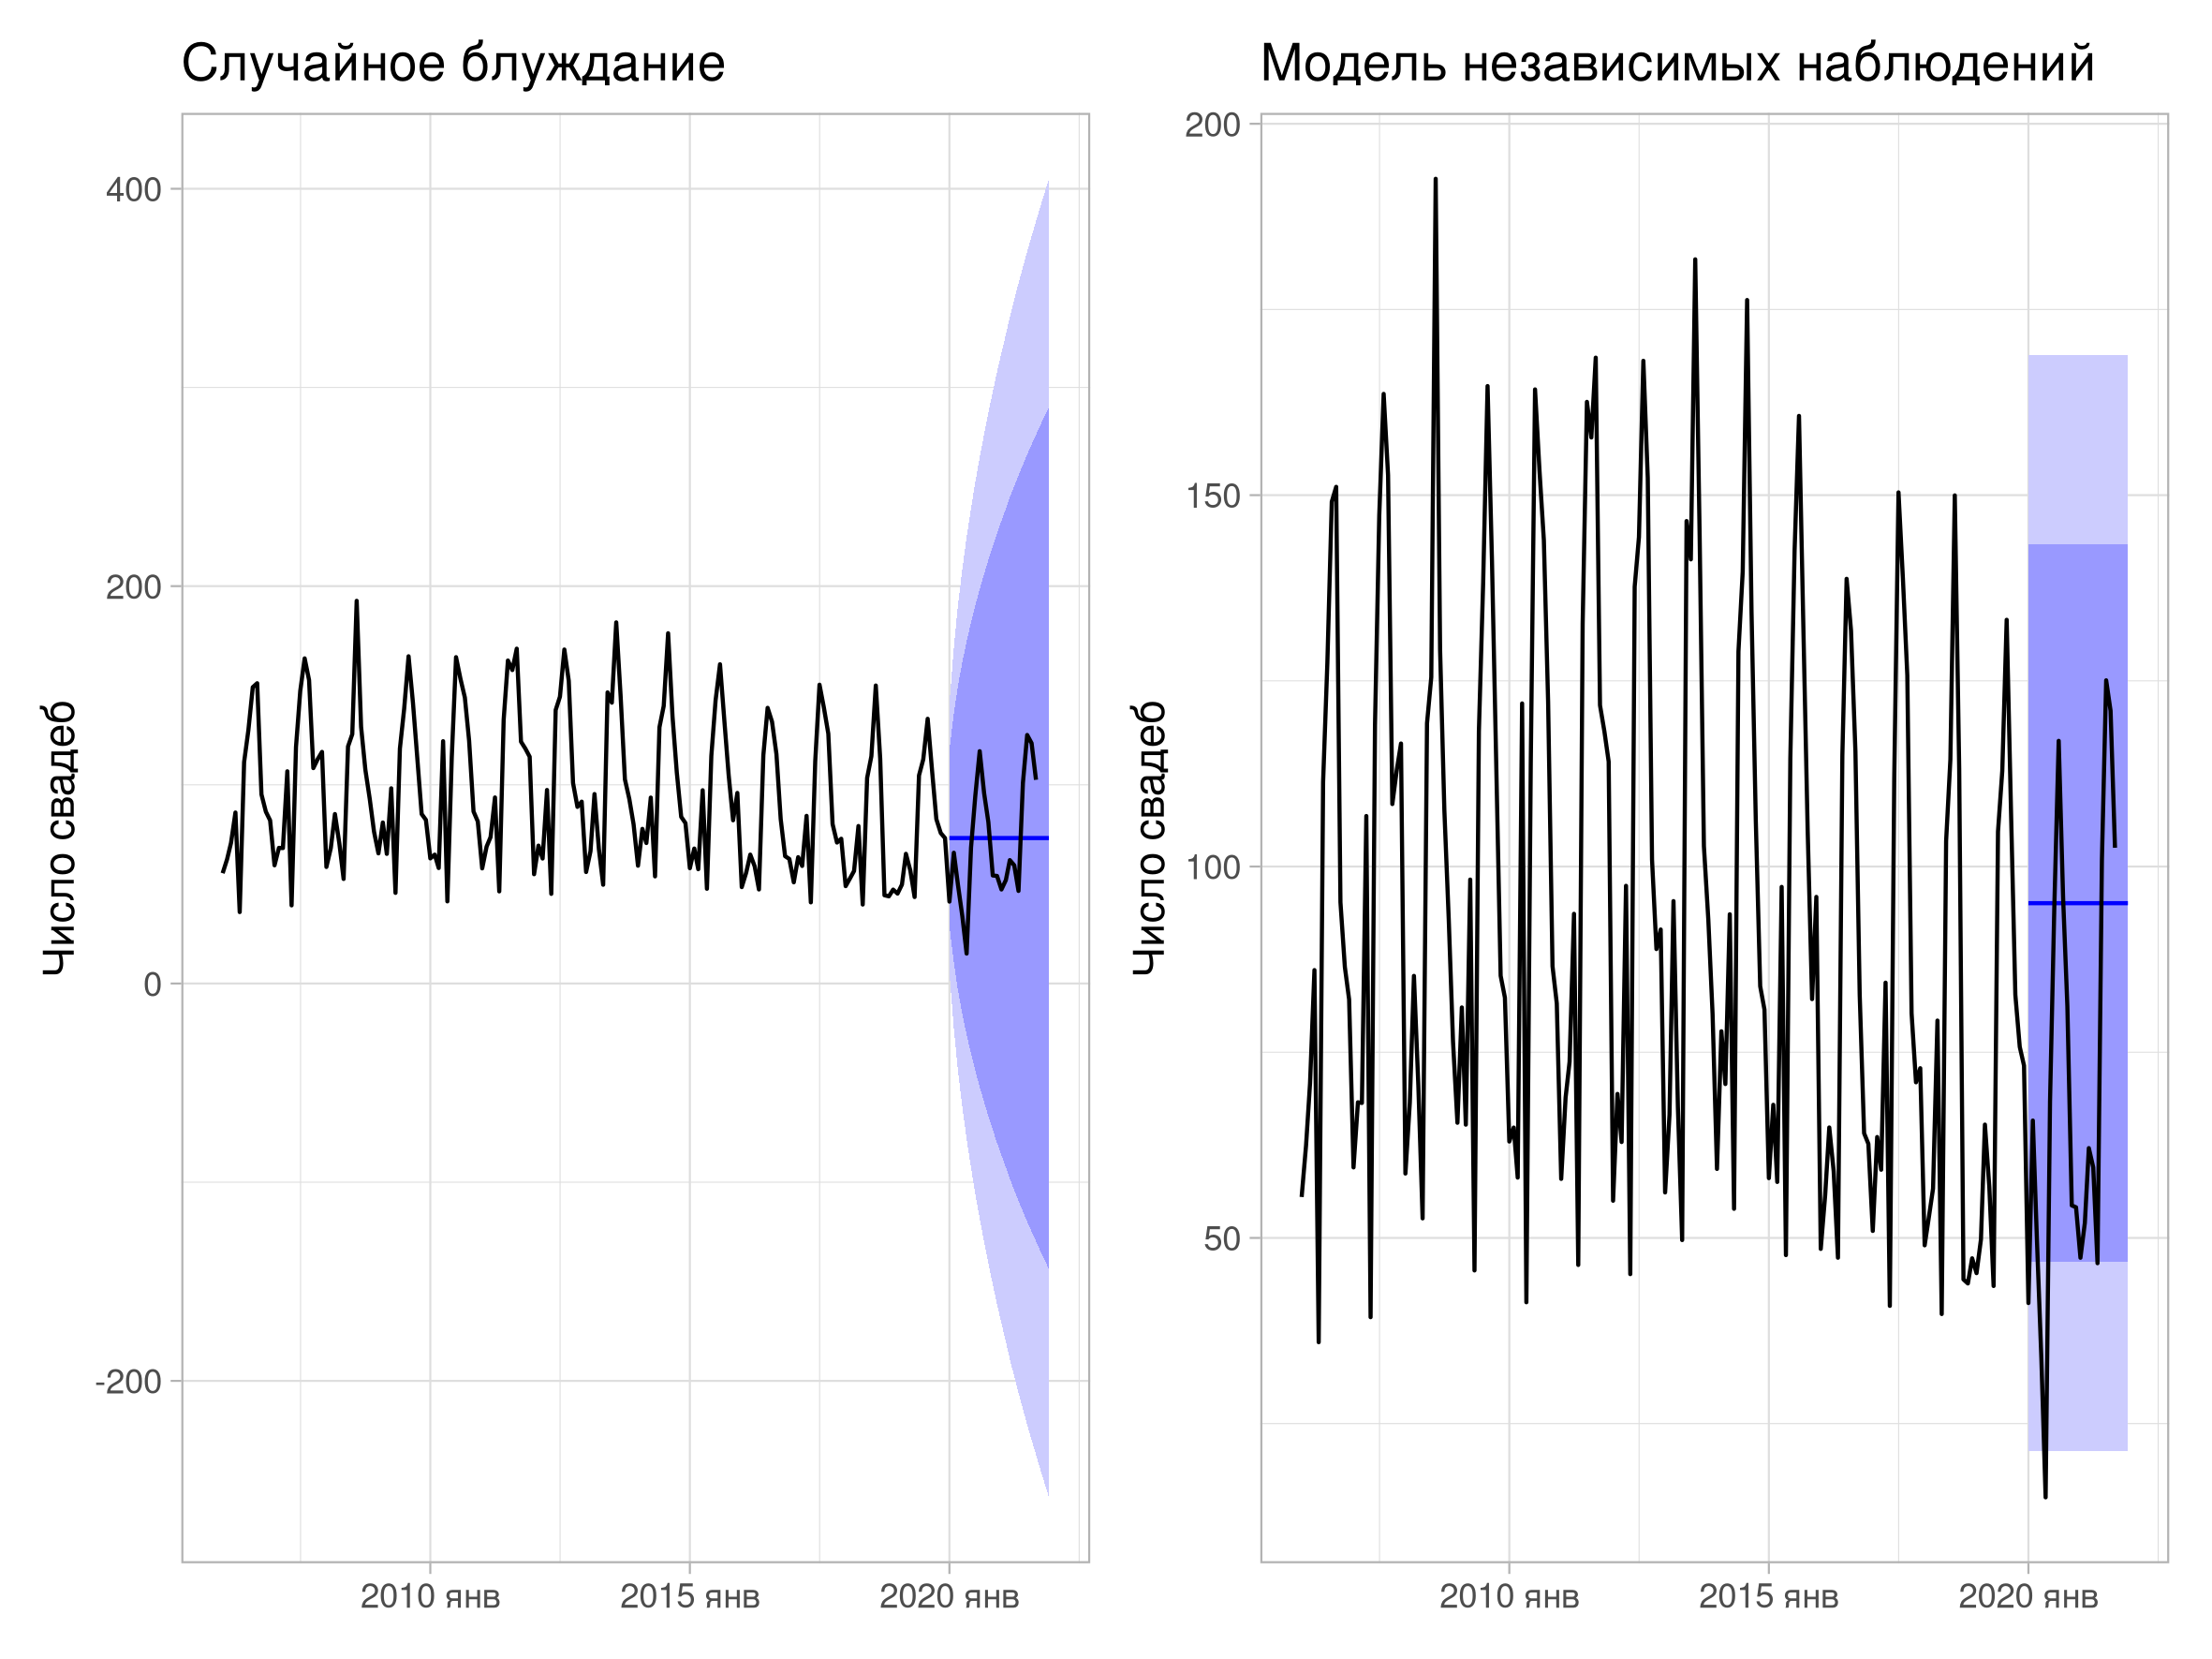
\includegraphics[width=\textwidth]{pictures/om_ts_01-157.png}

\end{frame}


\begin{frame}{Сезонное случайное блуждание}

  \begin{block}{Сезонная наивная модель}
  \[
  y_t = y_{t-12} + u_t,  
  \]
  где $u_t$ — белый шум, $u_t \sim \dN(0;\sigma^2)$, заданы $y_1$, \ldots, $y_{11}$.
  \end{block}
  \pause
  Переформулируем: $y_t - y_{t-12} = \Delta_{12} y_t = u_t$.
  \pause
  \alert{Оценки:}
  \[
  \hat\sigma^2_{ML} = \frac{\sum(\Delta_{12} y_i - \overline {\Delta_{12} y})^2}{T - 12}.  
  \]
  \pause
  \alert{Интервальный прогноз} на $h$ \alert{сезонов} вперёд:
  \[
  [y_{T} - 1.96 \hat \sigma \sqrt{h}; y_{T} + 1.96 \hat \sigma  \sqrt{h}]  
  \]
\end{frame}

\begin{frame}{Уже неплохо!}

  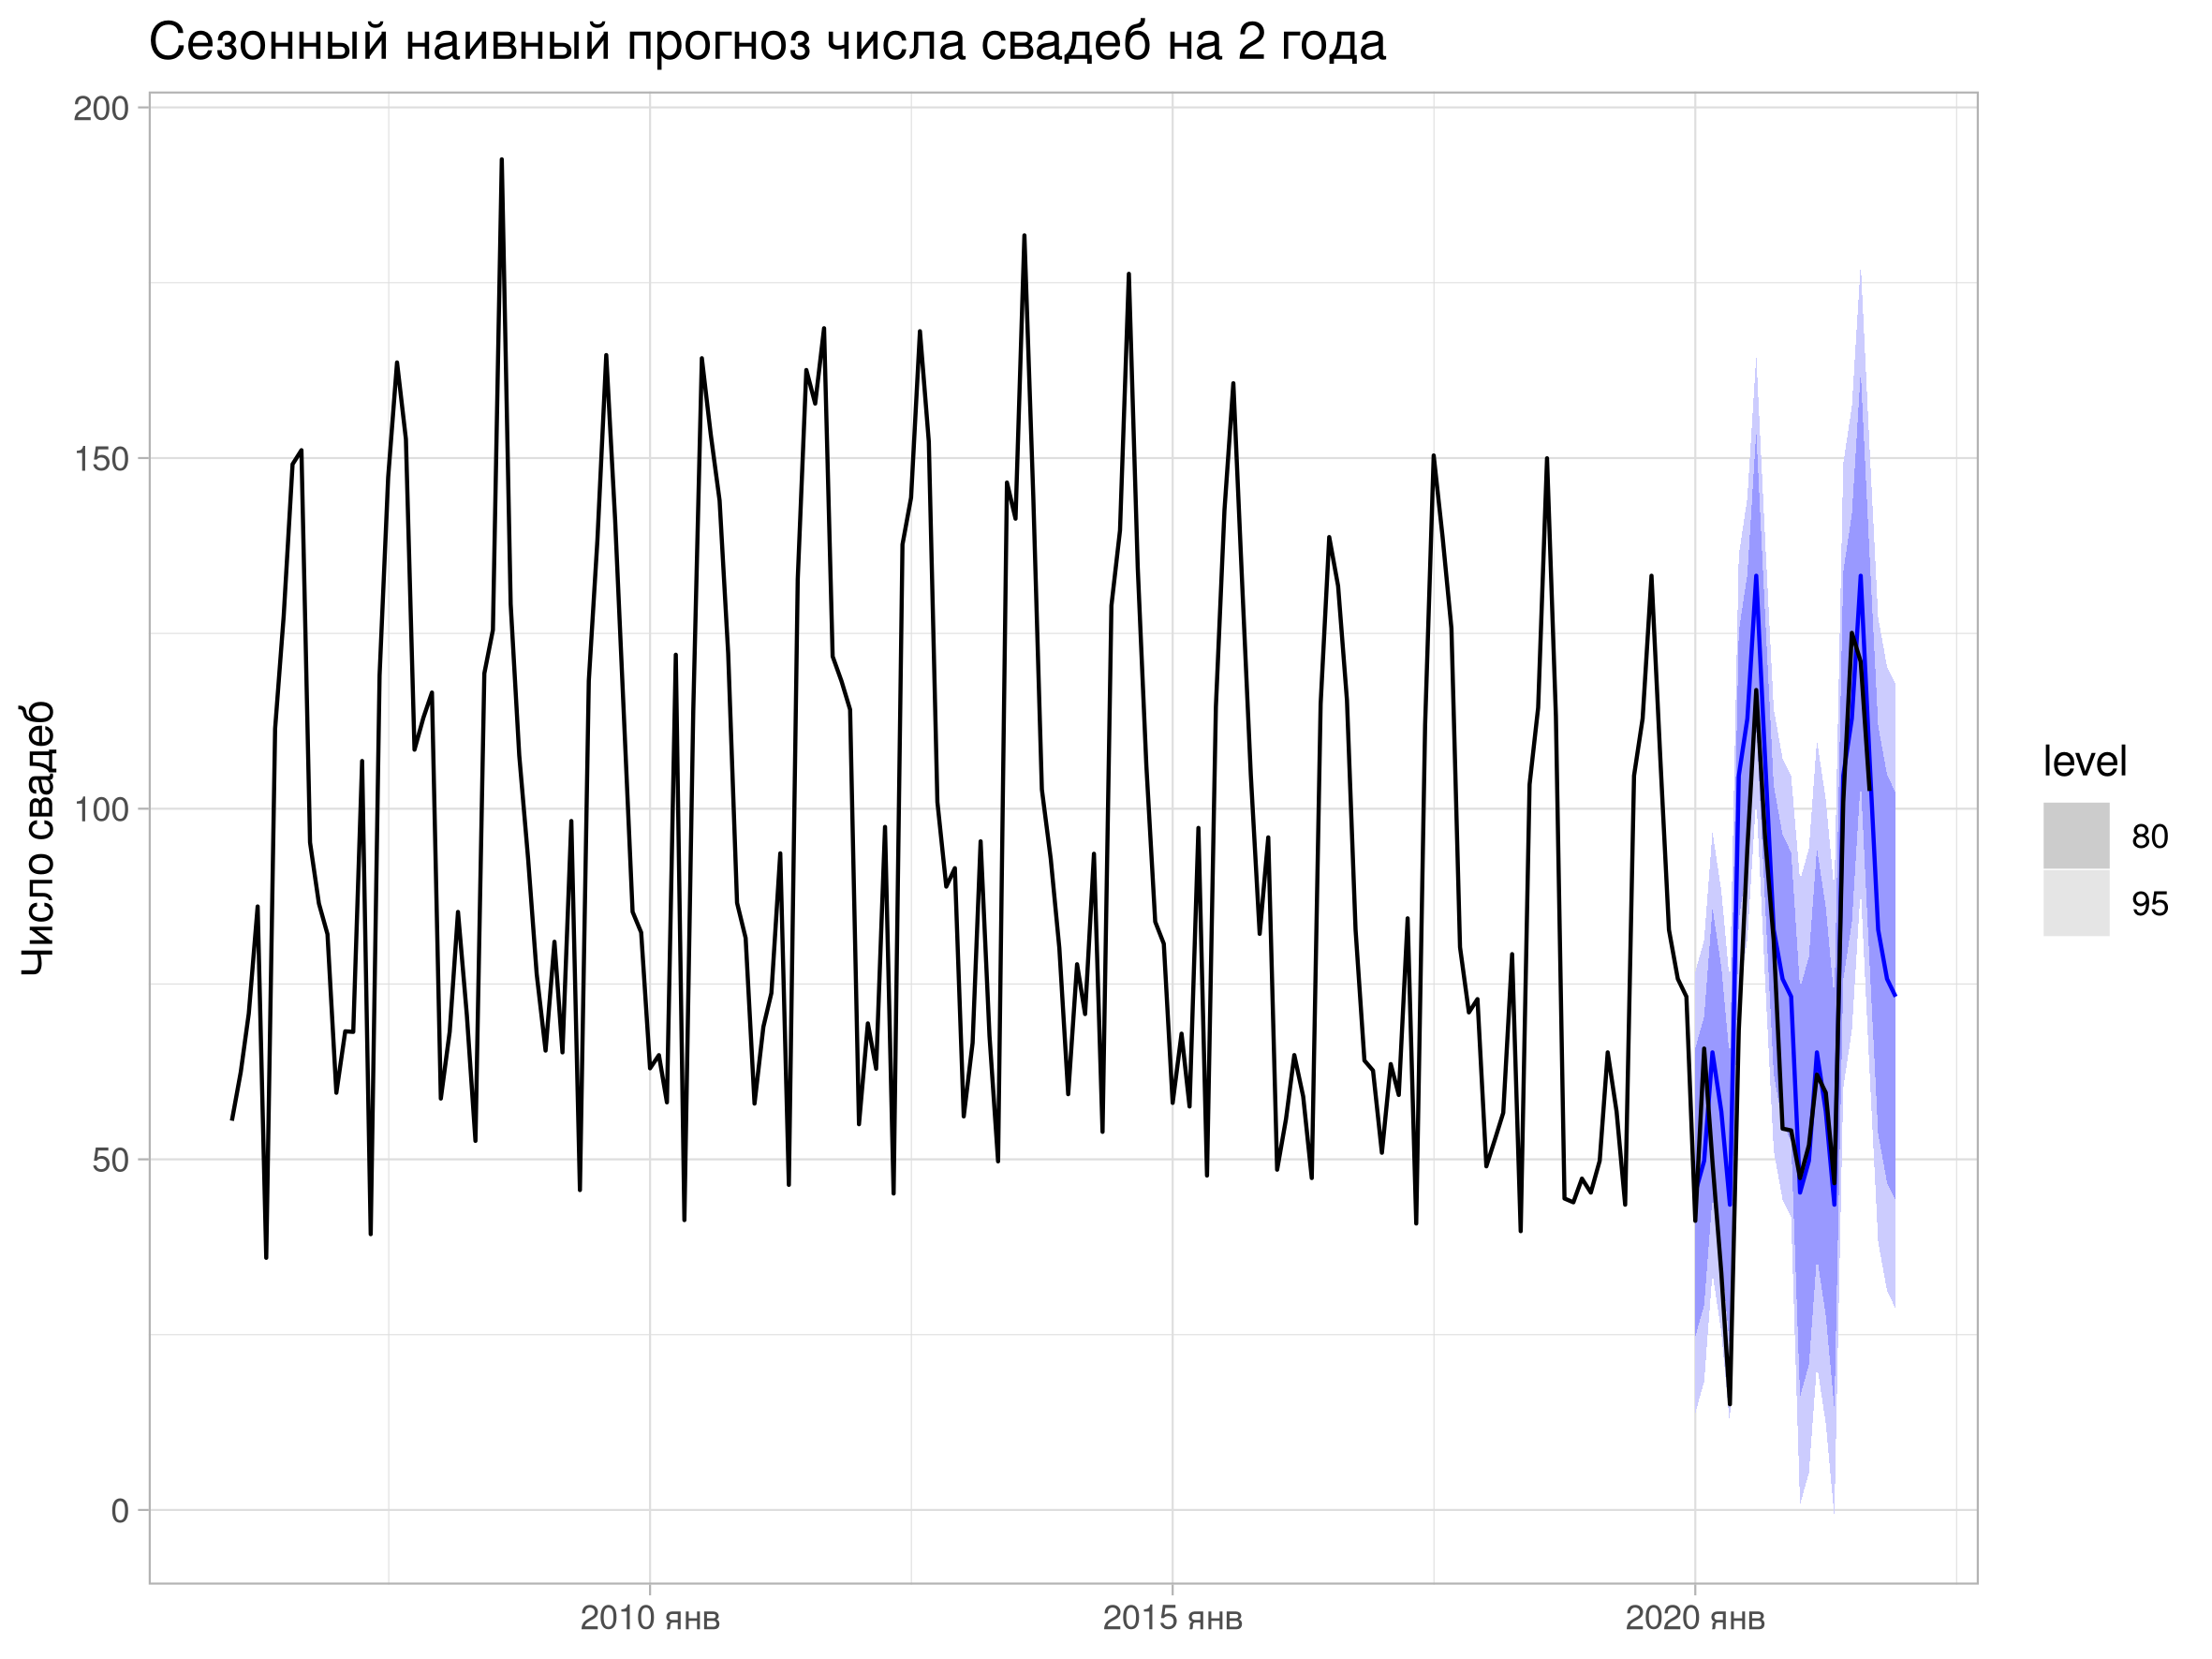
\includegraphics[width=\textwidth]{pictures/om_ts_01-162.png}


\end{frame}


\begin{frame}
  \frametitle{Зачем нужны наивные модели?}

  \begin{itemize}[<+->]
    \item \alert{Идеи} для сложных моделей.
    
    Модели \alert{стационарных рядов} похожи на модель независимых наблюдений. 

    Модели \alert{нестационарных рядов} похожи на случайное блуждание. 

    \item \alert{База для сравнения}. 
    
    При оценке сложной модели очень важно иметь базу сравнения. 

    \item \alert{Помощники} других моделей. 
    
    Можно \alert{усреднить прогнозы} сложной модели и наивной сезонной!
  \end{itemize}
  

\end{frame}

\begin{frame}{Наивные модели: итоги}

  \begin{itemize}[<+->]
    \item Белый шум — то, что не охота моделировать. 
    \item Независимые наблюдения и случайное блуждание.
    \item Идеи, составные части и помощники других моделей.
    \item База для сравнения.
  \end{itemize}
\end{frame}

